\section{Ziel}
    Ziel dieses Versuches ist es die Schichtdicke, den Brechungsindex und
    die Rauigkeit eines Polymerfilmes auf einem Silizium-Wafer zu bestimmen
    und ein allgemeines Verständnis für die Röntgenreflektometrie zu entwickeln.
\section{Theoretische Grundlagen}
    \subsection{Funktionsweise einer Röntgenröhre}
        Der Aufbau einer Elektronenröhre zur Erzeugung von Röntgenstrahlung ist in Abbildung \ref{fig:Rohr} dargestellt.
        Eine Kathode wird durch eine Heizspannung $U_H$ erhitzt und emittiert daraufhin Elektronen.
        Diese werden in dem elektrischen Feld einer angelegten Beschleunigungsspannung $U_B$ zur Anode hin beschleunigt.
        Beim Auftreffen der Elektronen wird elektromagnetische Strahlung im Röntgenbereich ausgesendet.
        Diese setzt sich prinzipiell aus zwei Komponenten zusammen.
        \begin{figure}[h]
            \centering
            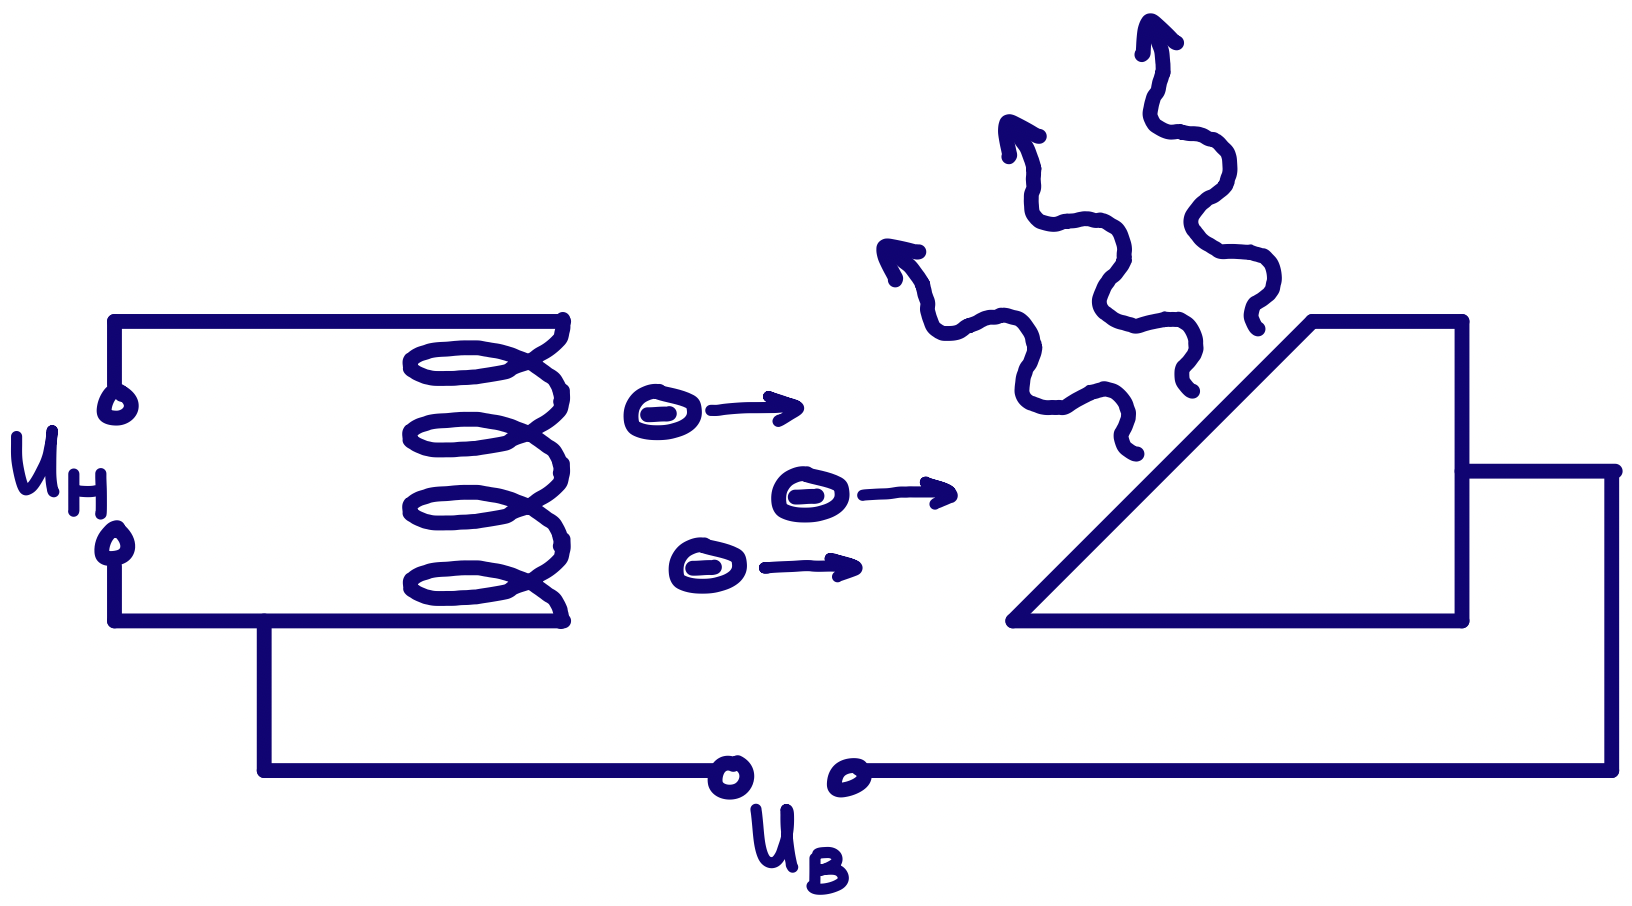
\includegraphics[width = 0.7\textwidth]{pictures/Rohr.png}
            \caption{Schematischer Aufbau einer Röntgenröhre einschießlich der Heizkathode und
                        der Anode aus welcher die Röntgenstrahlung emittiert wird.
                        $U_H$ bezeichnet die Heizspannung, welche zum Auslösen der Elektronen benötigt wird und
                        $U_B$ die Spannung die zum Beschleunigen dieser benutzt wird.}
            \label{fig:Rohr}
        \end{figure}
        Einerseits tritt die sogennante "'charakteristische Röntgenstrahlung"' auf.
        Diese entsteht, wenn die beschleunigten Elektronen in der Anode Elektronen aus den innersten Schalen herausschlagen.
        Die resultierenden leeren Plätze werden daraufhin von Elektronen aus höherenergetische Schalen gefüllt und die Energiedifferenz
        der zwei am Übergang teilnehmenen Schalen wird in Form eines (Röntgen-)Photons ausgesendet.
        So treten diskrete Linien im Röntgenspektrum auf, die den Photonen aus diesen Übergängen entsprechen.

        Andererseits taucht im Spektrum der Röntgenstrahlung ebenfalls ein energetisch kontinuierlicher Anteil auf.
        Dieser ist zurückzuführen auf das Abbremsen, was die Elektronen erfahren, wenn sie in das Anodenmaterial eindringen.
        Da jedes Elektron unterschiedlich stark abgebremst wird, bevor es das Anodenmaterial ionisiert,
        entsteht hierbei kein diskretes, sondern ein kontinuierliches Spektrum, welches "Bremsspektrum" genannt wird.
    \subsection{Reflexion und Brechung von Licht}
        Kommt eine elektromagnetische Welle aus dem Vakuum mit einem Brechungsindex $n_{Vakuum}=0$ und trifft auf ein glattes homogenes Medium unter einem Winkel $\alpha_i$,
        so wird ein Teil der Gesamtintensität der Strahlung unter einem Winkel $\alpha_r=\alpha_i$ reflektiert und
        der andere Teil transmittiert und gebrochen unter dem Winkel $\alpha_r$ in Abhängigkeit der Brechungsindizes $n$
        des Mediums, der gegeben ist als
        \begin{equation}
            n=1-\delta - \text{i}\beta \, .
        \end{equation}
        Dabei trägt die im Material vorliegende Dispersion $\delta$ zum Realteil des Brechungsindizes und die Absorption $\beta$ zum Imaginärteil bei.
        Die Absorption liegt im Größenordnungsbereich von $10^{-9}$ und berechnet sich über
        \begin{equation}
            \beta = \frac{\lambda\mu}{4\pi} \, ,
            \label{eqn:beta}
        \end{equation}
        wobei $\mu$ den linearen Absorptionskoeffizienten und $\lambda$ die Wellenlänge der einfallenden Strahlung beschreibt.
        Röntgenlicht besitzt in Materie einen Brechungsindex $n<1$, was jedes Medium für Röntgenstrahlung optisch dünner erscheinen lässt als Vakuum
        und ermöglicht Totalreflexion, wenn der Einfall möglichst flach unterhalb eines kritischen Winkels $\alpha_c$ auf die Ebene erfolgt.

        Die jeweiligen Reflexions- bzw. Transmissionskoeffizienten beim Übergang von Vakuum zu einem Medium des Brechungsindex $n$
        sind gegeben durch die Fresnel'schen Gleichungen. Dabei wird unterschieden zwischen einer Polarisation senkrecht zur Einfallsebene und eine Polarisation parallel zur Einfallsebene.
        Die Unterscheidung wird allerdings aufgehoben, da für Röntgenstrahlen die Brechungsindizes $n$ nahezu gleich sind und somit die Gleichungen reduziert werden auf die folgenden zwei:
        \begin{align}
            t&=\frac{2n_1\sin\alpha_i}{n_1\sin\alpha_i+n_2\sin\alpha_t} \\
            r&=\frac{n_1\sin\alpha_i-n_2\sin\alpha_t}{n_1\sin\alpha_i+n_2\sin\alpha_t}
        \end{align}
        Im Rahmen der Röntgenreflektometrie wird das Intensitätsverhältnis zwischen eingehendem und reflektierten Strahl gemessen.
        Diese sogennante Fresnel-Reflektivität ergibt sich durch
        \begin{equation}
            R_F=\vert r\vert^2=\frac{\left(\alpha_i-p_+\right)^2+p_-^2}{\left(\alpha_i+p_+\right)^2+p_-^2}
            \label{eqn:R_F}
        \end{equation}
        mit
        \begin{equation}
            p_\pm^2=\frac{1}{2}\left(\sqrt{\left(\alpha_i^2-\alpha_c^2\right)^2+4\beta^2}\pm\left(\alpha_i^2-\alpha_c^2\right)\right) \, .
            \label{eqn:p}
        \end{equation}
    \subsection{Kiessig-Oszillationen}
    \label{sec:KO}
        Wird die Schicht eines beliebigen Materials auf einem Substrat betrachtet und die Reflektivität gemessen,
        so fällt auf, dass diese innerhalb der, ab einem bestimmten kritischen Einfallswinkel $\alpha_c$,
        abfallenden Kurve zusätzlich oszilliert.
        Das lässt sich darauf zurückführen, dass der Röntgenstrahl sich zunächst am Vakuum-Medium Übergang
        aufteilt in einen reflektierten und einen transmittiert-gebrochenen Anteil.
        Dieser Vorgang ist schematisch in Abbildung \ref{fig:Kiessig} schematisch dargestellt.
        \begin{figure}[h]
            \centering
            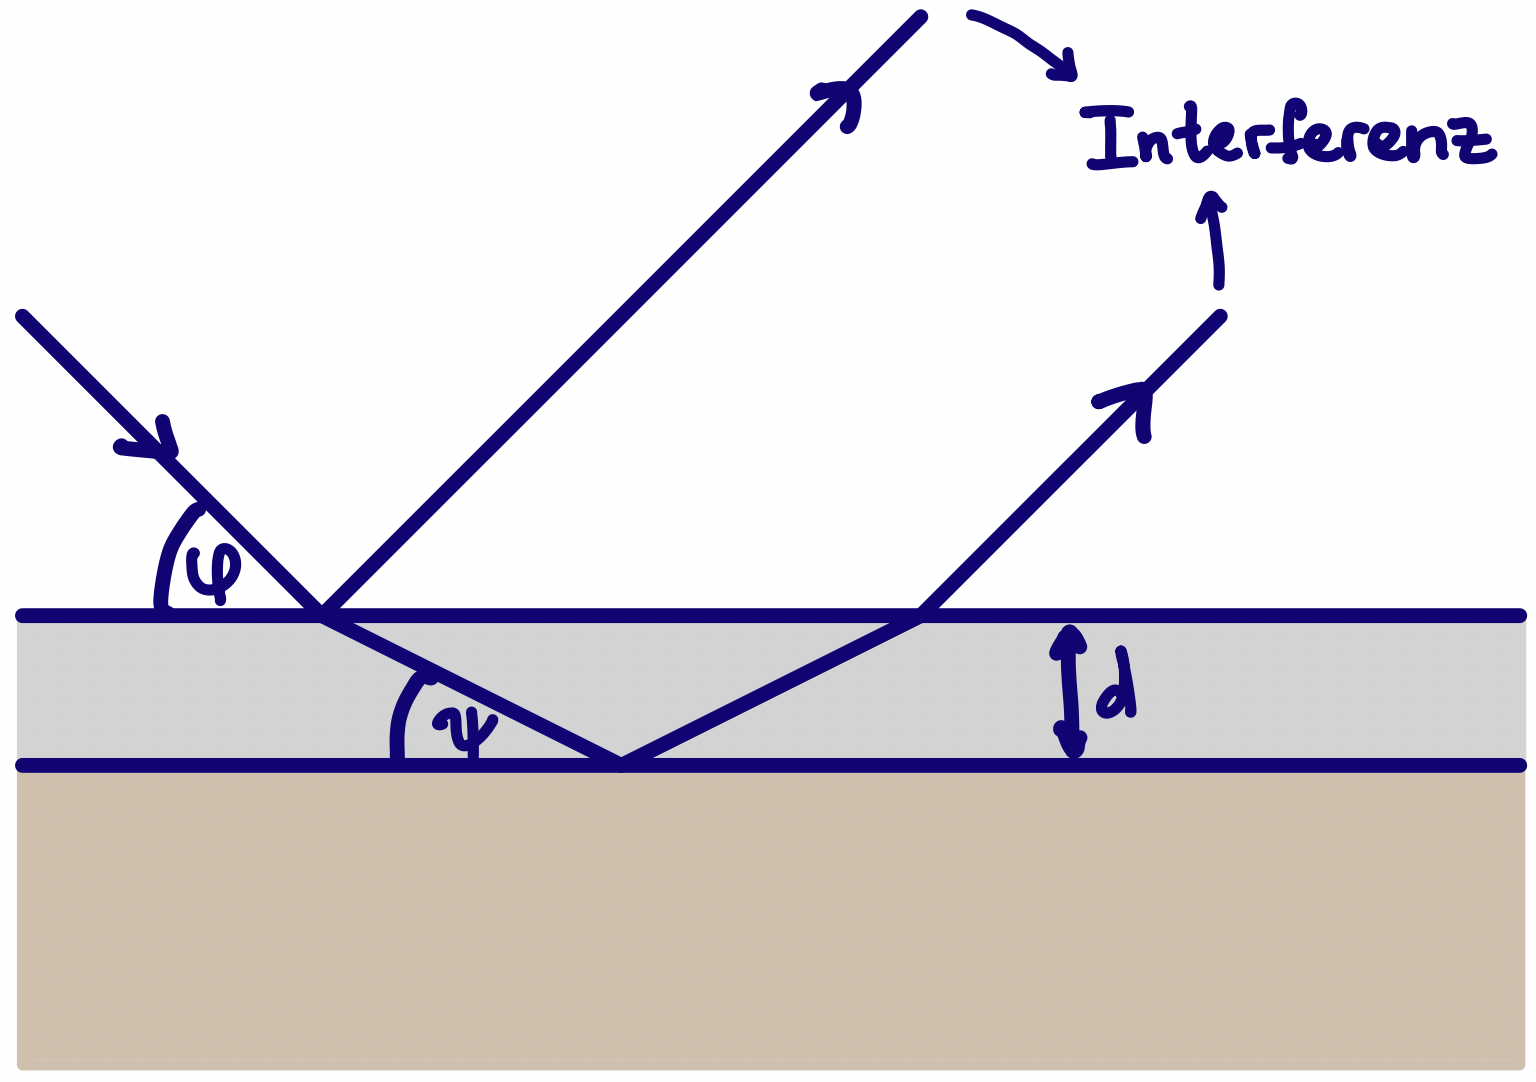
\includegraphics[width = 0.7\textwidth]{pictures/Kiessig.png}
            \caption{Skizze des Entstehungsprozesses der Kiessig-Oszillationen an einer Schicht (grau) der Dicke $d$ auf einem Substrat (braun).
                        Der Röntgenstrahl trifft unter einem Winkel $\varphi$ auf die Probe und wird teilweise reflektiert und teilsweise gebrochen,
                        sodass er dann im Winkel $\psi$ am Substrat reflektiert wird und nach erneuter Beugung an der Oberfläche wieder im Winkel $\varphi$ austritt.}
            \label{fig:Kiessig}
        \end{figure}
        Letzterer wird nach Durchqueren der Schicht an dem Substrat reflektiert und beim Übergang zurück ins Vakuum erneut gebrochen,
        sodass er wieder parallel zum direkt reflektierten Strahl ist.
        Diese beiden Röntgenwellen interferieren daraufhin entweder konstruktiv oder destruktiv untereinander
        in Abhängigkeit der Phasenverschiebung, welche sich zwischen den Strahlen ergibt.
        Beim Erhöhen des Einfallwinkels entstehen sogenannte "Kiessig-Osszilation".
        In Abbildung \ref{fig:Oszi} sind sowohl die theoretische Fresnel-Reflektivität als auch die Kiessig-Osszilationen
        beispielhaft für eine Polystyrolschicht auf einem Silizium-Substrat zu sehen.
        \begin{figure}[h]
            \centering
            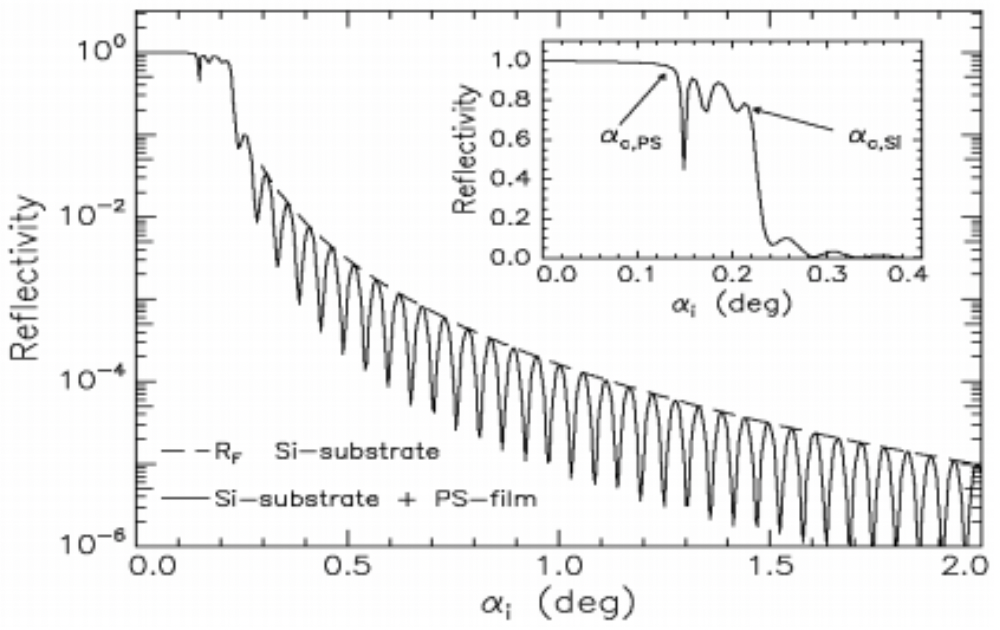
\includegraphics[width = 0.7\textwidth]{pictures/Oszi.png}
            \caption{Fresnel-Reflektivität in Abhängigkeit vom Einfallswinkel einer Polystyrolschicht auf einem Siliziumwafer.
                        Der Einsatz zeigt vergrößert den Bereich bis $\alpha_i<0,4°$,
                        wo deutliche Abfälle der Reflektivität zu erkennen sind
                        an den Winkeln $\alpha_{c,Si}$ und $\alpha_{c,PS}$,
                        welche jeweils den kritischen Winkeln des Silizium-Substrates
                        und der Polysteren-Schicht entsprechen. Entnommen aus \cite{tolan_x-ray_1999}.}
            \label{fig:Oszi}
        \end{figure}
        Da die Phasenverschiebung von der Schichdicke $d$, als auch dem Brechungsindex $n$ der Schicht abhängt,
        ist es möglich diese zu bestimmen
        \begin{align}
            \delta&=\frac{1}{2}\frac{\alpha_{i1}^2m_2^2-\alpha_{i2}^2m_1^2}{m_2^2-m_1^2} \\
            d&=\frac{\lambda}{2\Delta\alpha_i} \, , 
            \label{eqn:d_alpha}
        \end{align}
        wenn die Ordnungszahl $m$ und der Einfallswinkel $\alpha_i$ zweier Minima bekannt ist.
        \subsubsection{Parratt-Algorithmus}
            Im Falle eines Mehrschichtsystems (siehe Abbildung \ref{fig:Parratt}) liegt zwischen je zwei benachbarten Schichten eine Reflexion-Transmission Beziehung vor wie in \ref{sec:KO} beschrieben.
            Die entstehenden Kiessig-Oszillationen überlagern in diesem Fall und es wird sehr schwer Aussagen über die einzelnen Schichten zu treffen.
            Zur Beschreibung eines solchen Systems wurde der sogenannte "Parratt-Algorithmus" eingeführt.
            \begin{figure}[h]
                \centering
                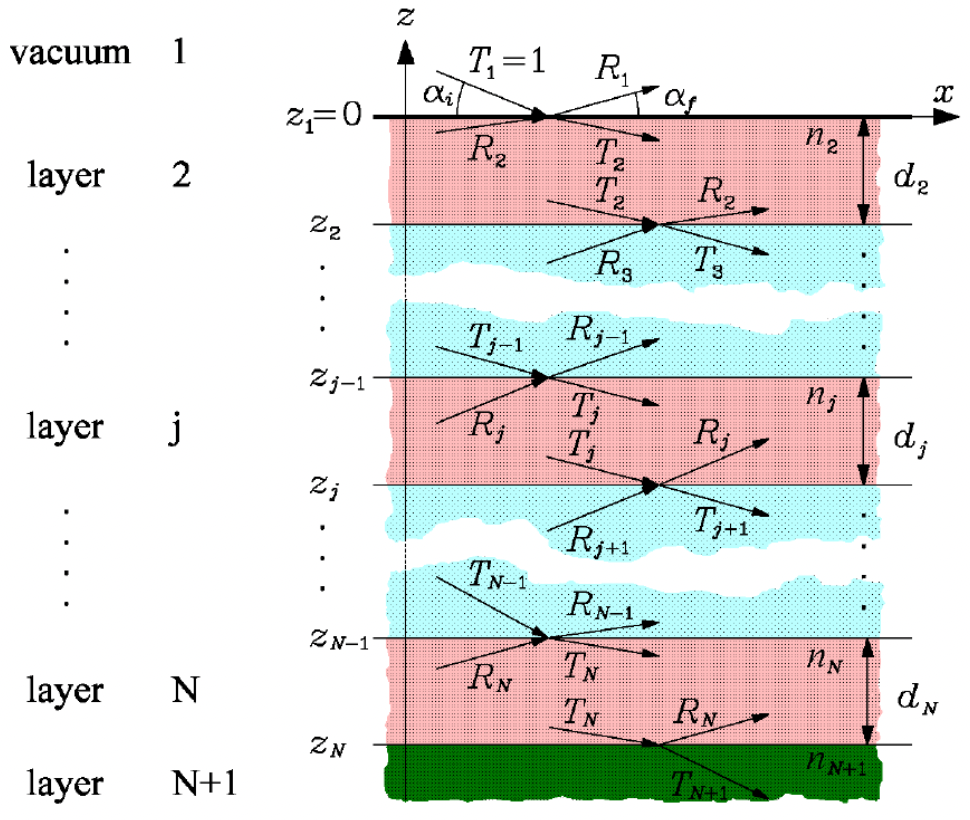
\includegraphics[width = 0.7\textwidth]{pictures/Parratt.png}
                \caption{Mehrschichtsystem aus $N$ Grenzflächen mit Schichten verschiedener Brechungsindizes $n$ und Dicken $d$ auf einem Substrat.
                        Für jede Schicht sind die reflektierten und transmittierten Amplituden $R_j$ und $T_j$ eingetragen. Entnommen aus \cite{e1_tu_dortmund_versuchsanleitung_nodate}.}
                \label{fig:Parratt}
            \end{figure}
            Dazu wird an jeder Grenzschicht die Wechselwirkung zwischen Röntgenstrahlung und Medium mittels den Fresnel'schen Gleichungen beschrieben
            und ausgehend von dem Substrat das Amplitudenverhältnis zwischen reflektierter und transmittierter Welle rekursiv berechnet.
            Dabei wird als Randbedingung angenommen, dass die aus dem Vakuum kommende Welle noch keine Grenzfläche passiert hat ($T_1=1$)
            und dass das Substrat im Vergleich zu den einzelnen Schichten unendlich lang ist ($d_{N+1}\gg d_j$) und dementsprechend $R_{N+1}=0$ gilt.
            Es ergibt sich
            \begin{equation}
                X_j=\frac{R_N}{T_N}=\exp\left(-2ik_{z,j}z_j\right)\cdot\frac{r_{j,j+1}+X_{j+1}\exp\left(-2ik_{z,j+1}z_j\right)}{1+r_{j,j+1}X_{j+1}\exp\left(-2ik_{z,j+1}z_j\right)} \, ,
                \label{eqn:X_j}
            \end{equation}
            wobei
            \begin{equation}
                k_{z,j}=\frac{2\pi}{\lambda}\cdot\sqrt{n_j^2-\cos\alpha_i^2}
                \label{eqn:k_z}
            \end{equation}
            die $z$-te Komponente des $j$-ten Wellenvektors ist.
            Der Exponentialterm wird Phasenfaktor genannt und ist von der Schichttiefe $z_j$ abhängig und
            die im Bruch der Formel vorkommenden Fresnel-Koeffizienten $r$ von der Disperion $\delta$ und damit vom Brechungsindex $n$.
            Aus dem Amplitudenverhältnis kann letztendlich die Fresnel-Reflektivität
            \begin{equation}
                R_F=\vert X_1\vert^2=\frac{\vert R_1\vert^2}{\vert T_1\vert^2}=\vert R_1\vert^2
                \label{eqn:R_F_parratt}
            \end{equation}
            berechnet werden.
        \subsubsection{Rauigkeitkorrektur}
            Da komplett glatte Oberflächen in der Natur nicht vorkommen, wird eine Korrektur eingeführt, um die Rauigkeit dieser mit einzubeziehen.
            Ein Maß für die Rauigkeit der $j$-ten Grenzfläche ist gegeben durch
            \begin{equation}
                \sigma_j^2=\int \left(z-z_j\right)\cdot P_j(z) \,dz \, ,
            \end{equation}
            wobei die $z(x,y)$-Koordinaten durch eine Wahrscheinlichkeitsdichtefunktion $P_j(z)$ gewichtet werden.
            Damit werden die Fresnel-Koeffizienten unter der Bedingung, dass $\sigma\ll d$,
            also dass die Rauigkeit klein ist im Gegensatz zur Schichtdicke, modifiziert zu
            \begin{align}
                \tilde{r}_{j,j+1}&=r_{j,j+1}\cdot\exp\left(-2k_{z,j}k_{z,j+1}\sigma_j^2\right) \\
                \tilde{t}_{j,j+1}&=t_{j,j+1}\cdot\exp\left(\frac{1}{2}\left(k_{z,j}-k_{z,j+1}\right)^2\sigma_j^2\right)
                \label{eqn:r_rau}
            \end{align}
            und in den Parratt-Algorithmus eingebunden.